\documentclass[handout,compress]{beamer}

\usetheme[block=fill]{metropolis}

\usepackage{graphicx} % Allows including images
\usepackage{amsmath,amsfonts,amsthm,amssymb}
\usepackage{color}
\usepackage{xcolor,cancel}
%\setitemize{label=\usebeamerfont*{itemize item}%
%	\usebeamercolor[fg]{itemize item}
%	\usebeamertemplate{itemize item}}
\definecolor{mDarkBrown}{HTML}{604c38}
\definecolor{mDarkTeal}{HTML}{23373b}
\definecolor{mLightBrown}{HTML}{EB811B}
\definecolor{mMediumBrown}{HTML}{C87A2F}
\definecolor{mygreen}{HTML}{98C2B9}
\definecolor{myyellow}{HTML}{DFD79C}
\definecolor{myblue}{HTML}{8CA7CC}
\definecolor{kern}{HTML}{8CC2B7}

\usepackage{float}
\usepackage{framed}
\usepackage{epsfig}
\usepackage{graphicx}
\usepackage{subcaption}
\usepackage{ulem}
\usepackage{hhline}
\usepackage{multirow}
\usepackage{comment}   
\usepackage{bbm}
\usepackage{tikz}   
\usepackage{ulem}
\def\Put(#1,#2)#3{\leavevmode\makebox(0,0){\put(#1,#2){#3}}}
\newcommand*\mystrut[1]{\vrule width0pt height0pt depth#1\relax}
\newcommand{\eqdef}{\mathbin{\stackrel{\rm def}{=}}}


\newcommand{\bs}[1]{\boldsymbol{#1}}
\newcommand{\bv}[1]{\mathbf{#1}}
\newcommand{\R}{\mathbb{R}}
\newcommand{\E}{\mathbb{E}}

\DeclareMathOperator*{\argmin}{arg\,min}
\DeclareMathOperator*{\argmax}{arg\,max}
\DeclareMathOperator{\nnz}{nnz}
\DeclareMathOperator{\Var}{Var}
\DeclareMathOperator{\sinc}{sinc}
\DeclareMathOperator{\mv}{mv}
\DeclareMathOperator{\sgn}{sgn}
\DeclareMathOperator{\step}{step}
\DeclareMathOperator{\gap}{gap}
\DeclareMathOperator{\poly}{poly}
\DeclareMathOperator{\tr}{tr}
\DeclareMathOperator{\orth}{orth}
\newcommand{\norm}[1]{\|#1\|}
\captionsetup[subfigure]{labelformat=empty}
\captionsetup[figure]{labelformat=empty}
\DeclareMathOperator*{\lmin}{\lambda_{min}}
\DeclareMathOperator*{\lmax}{\lambda_{max}}

\newcommand{\specialcell}[2][c]{%
  \begin{tabular}[#1]{@{}c@{}}#2\end{tabular}}
\newcommand{\specialcellleft}[2][c]{%
\begin{tabular}[#1]{@{}l@{}}#2\end{tabular}
}

\usepackage{tabstackengine}
\stackMath


%----------------------------------------------------------------------------------------
%	TITLE PAGE
%----------------------------------------------------------------------------------------

\title{CS-UY 4563: Lecture 5 \\ Model Selection and Regularization}
\author{NYU Tandon School of Engineering, Prof. Christopher Musco}
\date{}

\begin{document}

\begin{frame}
	\titlepage 
\end{frame}

\metroset{titleformat=smallcaps}

\begin{comment}
\end{comment}

\begin{frame}
	\frametitle{course admin}
	\begin{itemize}
		\item Multiple linear regression lab due \textbf{tomorrow night}. 
		\item Second written homework posted due \textbf{next Tuesday 2/18.} 
	\end{itemize}

Practice with gradients, function transformations, reduction from piecewise regression to multiple linear regression.
\begin{center}
	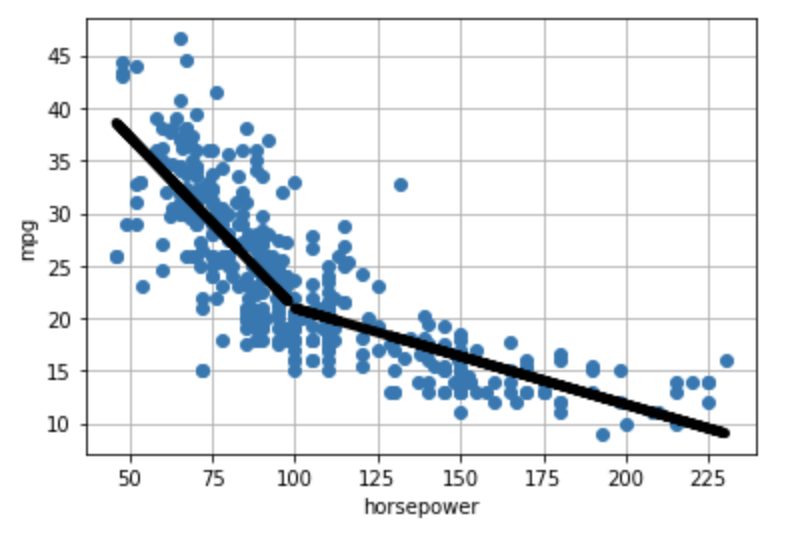
\includegraphics[width=.5\textwidth]{piecewise_fit.png}
\end{center}
\end{frame}

\begin{frame}
	\frametitle{course admin}
	\begin{itemize}
		\item TA office hours moved to \textbf{11am - 1pm in 219 Rogers Hall} -- this will be their permanent location. 
		\item I won't have office hours this week. 
	\end{itemize}
\end{frame}





\begin{frame}
	\frametitle{loss minimization}
	\textbf{Basic machine learning problem:}
	\begin{itemize}
		\item Given model $f_{\bs{\theta}}$ and \emph{loss function} $L_{\text{train}}(f_{\bs{\theta}})$. 
		\item Choose $\bs{\theta}^*$ to minimize $L_{\text{train}}(f_{\bs{\theta}})$. 
	\end{itemize}
\end{frame}

\begin{frame}
	\frametitle{model selection}
	\textbf{Model selection problem:}
	\begin{itemize}
		\item Given choice of many models $f_{\bs{\theta}_1}^{(1)}, f_{\bs{\theta}_2}^{(2)}, \ldots, f_{\bs{\theta}_q}^{(q)}.$
		\item Choose $\bs{\theta}_1^*, \ldots, \bs{\theta}_q^*$ to minimize $L_{\text{train}}(f_{\bs{\theta}_1}),\ldots, L_{\text{train}}(f_{\bs{\theta}_q})$. 
		\item Then choose the ``best'' model for our data. 
	\end{itemize}
\end{frame}

\begin{frame}
	\frametitle{model selection example}
	Polynomial regression models with different degree. 
	See \texttt{demo\_polyfit.ipynb}.
	\begin{center}
		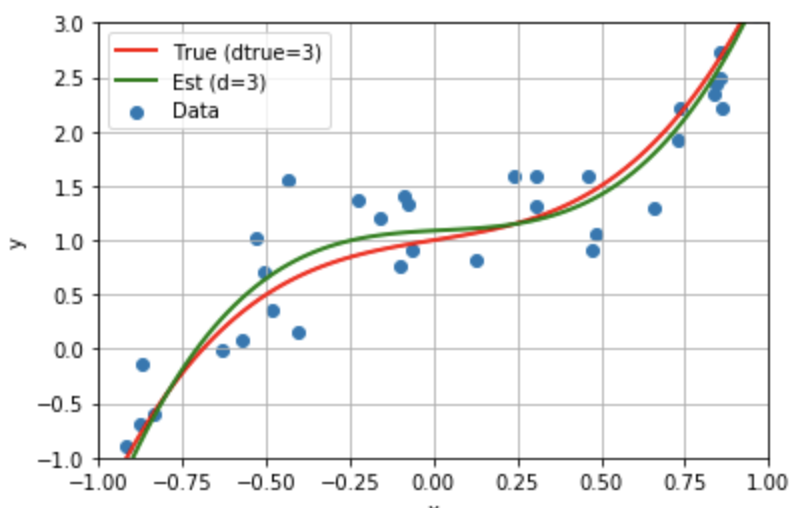
\includegraphics[width=.32\textwidth]{fit3.png}\includegraphics[width=.32\textwidth]{fit10.png}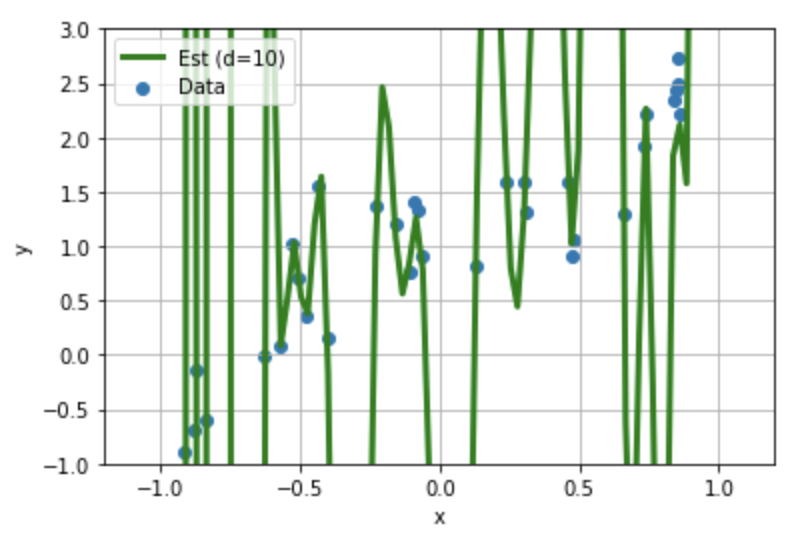
\includegraphics[width=.32\textwidth]{fit40.png}
	\end{center}
\begin{itemize}
	\item Model $f_{\bs{\theta}_1}^{(1)}$: all linear functions. 
	\item Model $f_{\bs{\theta}_2}^{(2)}$: all quadratic functions. 
	\item Model $f_{\bs{\theta}_3}^{(3)}$: all cubic functions. 
	\item $\ldots$
\end{itemize}
\end{frame}


\begin{frame}
	\frametitle{model selection example}
	\begin{center}
		\textbf{bag-of-words} models and \textbf{$\bv{n}$-grams}
	\end{center}
	Common way to represent documents (emails, webpages, books) as numerical data. The ultimate example of $1$-hot encoding.
	\begin{center}
		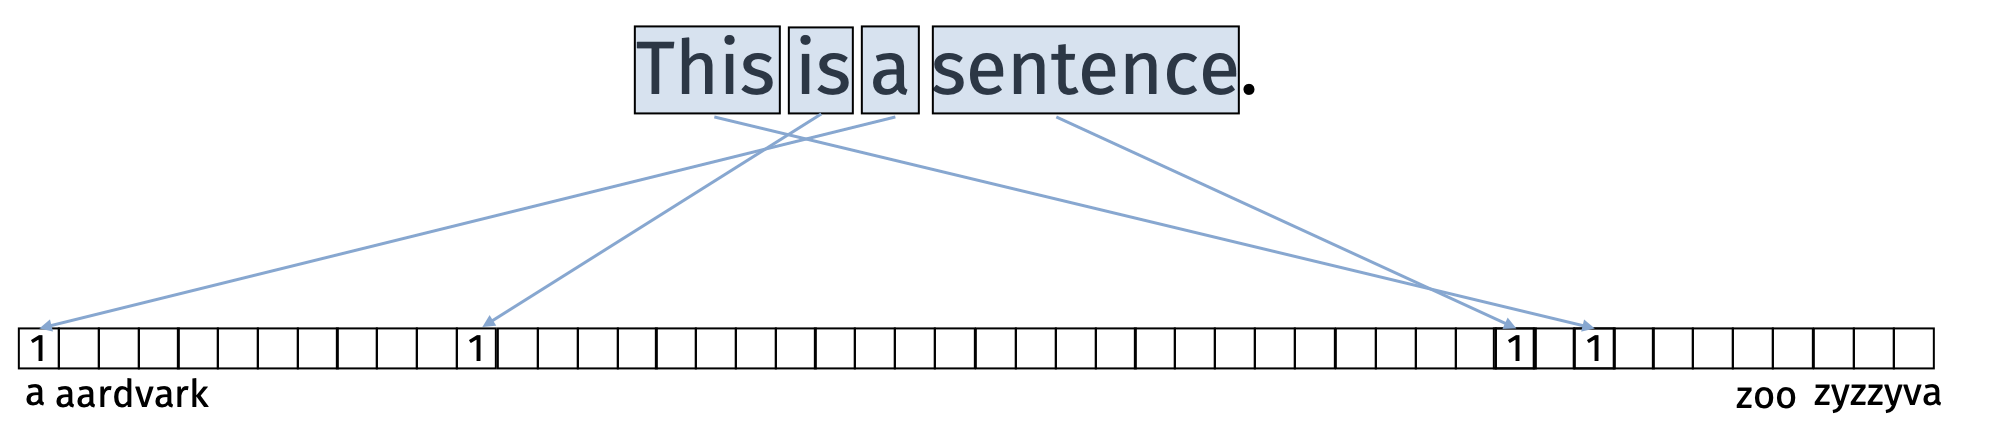
\includegraphics[width=\textwidth]{bagofwords.png}
		
		\alert{\Large \textbf{bag-of-words}}
	\end{center}
\end{frame}

\begin{frame}
	\frametitle{model selection example}
	\begin{center}
		\textbf{bag-of-words} models and \textbf{$\bv{n}$-grams}
	\end{center}
	Common way to represent documents (emails, webpages, books) as numerical data. The ultimate example of $1$-hot encoding.
	\begin{center}
		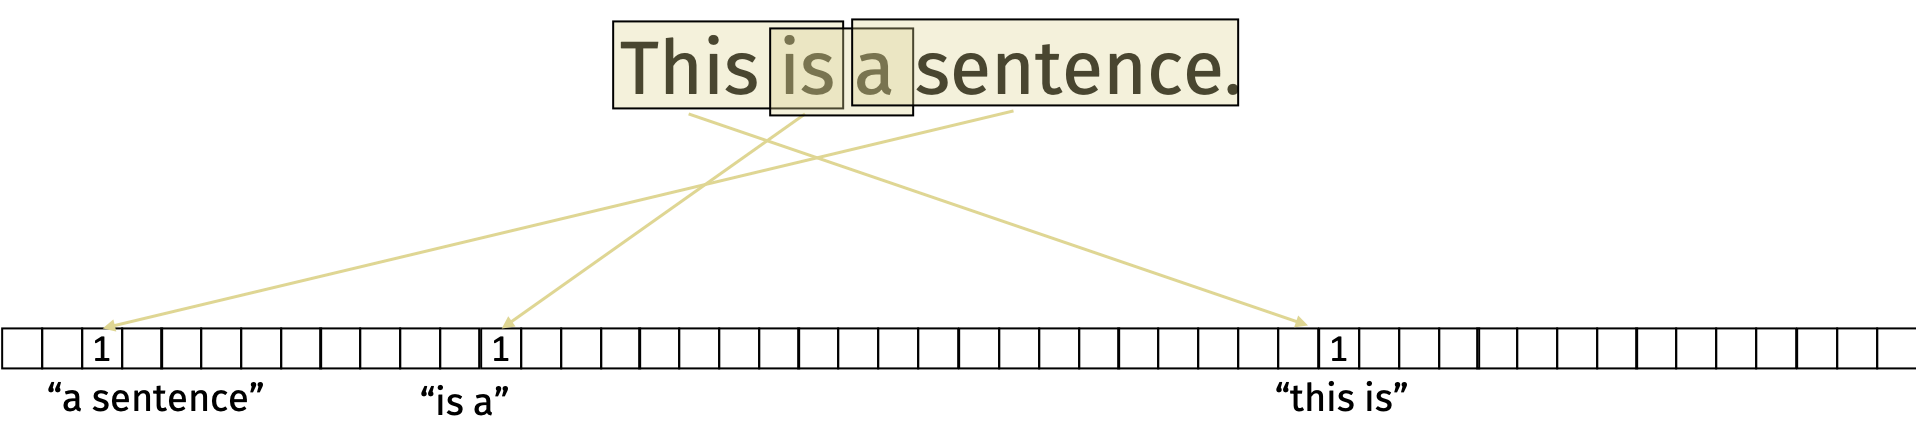
\includegraphics[width=\textwidth]{bigrams.png}
		
		\alert{\Large \textbf{bi-grams}}
	\end{center}
\end{frame}

\begin{frame}
	\frametitle{model selection example}
	\begin{center}
		\textbf{bag-of-words} models and \textbf{$\bv{n}$-grams}
	\end{center}
	Common way to represent documents (emails, webpages, books) as numerical data. The ultimate example of $1$-hot encoding.
	\begin{center}
		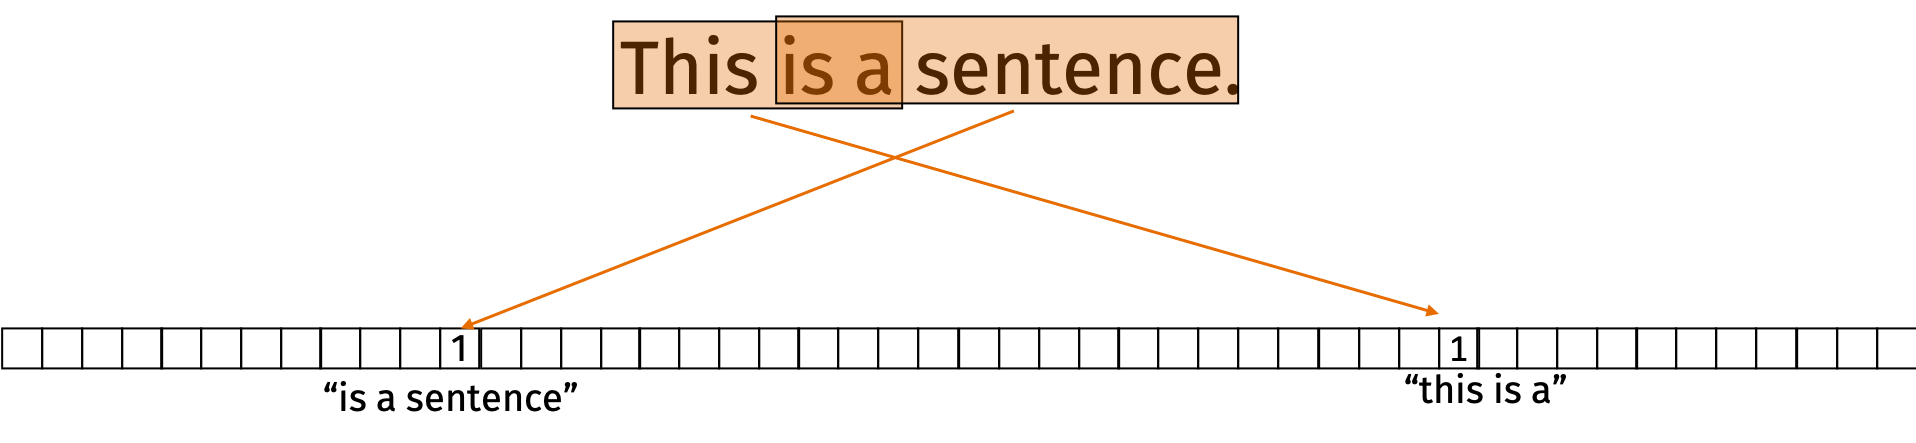
\includegraphics[width=\textwidth]{trigrams.png}
		
		\alert{\Large \textbf{tri-grams}}
	\end{center}
\end{frame}

\begin{frame}
	\frametitle{model selection example}
	\textbf{Models of increasing order:}
	\begin{itemize}
		\item Model $f_{\bs{\theta}_1}^{(1)}$: spam filter that looks at \textbf{single words}. 
		\item Model $f_{\bs{\theta}_2}^{(2)}$: spam filter that looks at \textbf{bi-grams}.
		\item Model $f_{\bs{\theta}_3}^{(3)}$: spam filter that looks at \textbf{tri-grams}.
		\item $\ldots$
	\end{itemize}
	\begin{center}
		``interest" \hspace{3em} ``low interest'' \hspace{3em}``low interest loan'' 
	\end{center}

	Increased length of \textbf{$\bv{n}$-gram} means more expressive power. 
\end{frame}

\begin{frame}[t]
	\frametitle{model selection example}
	\textbf{Electrocorticography ECoG (upcoming lab or demo):}
	\begin{itemize}
		\item Implant grid of electrodes on surface of the brain to measure electrical activity in different regions. 
	\end{itemize} 
	\begin{center}
		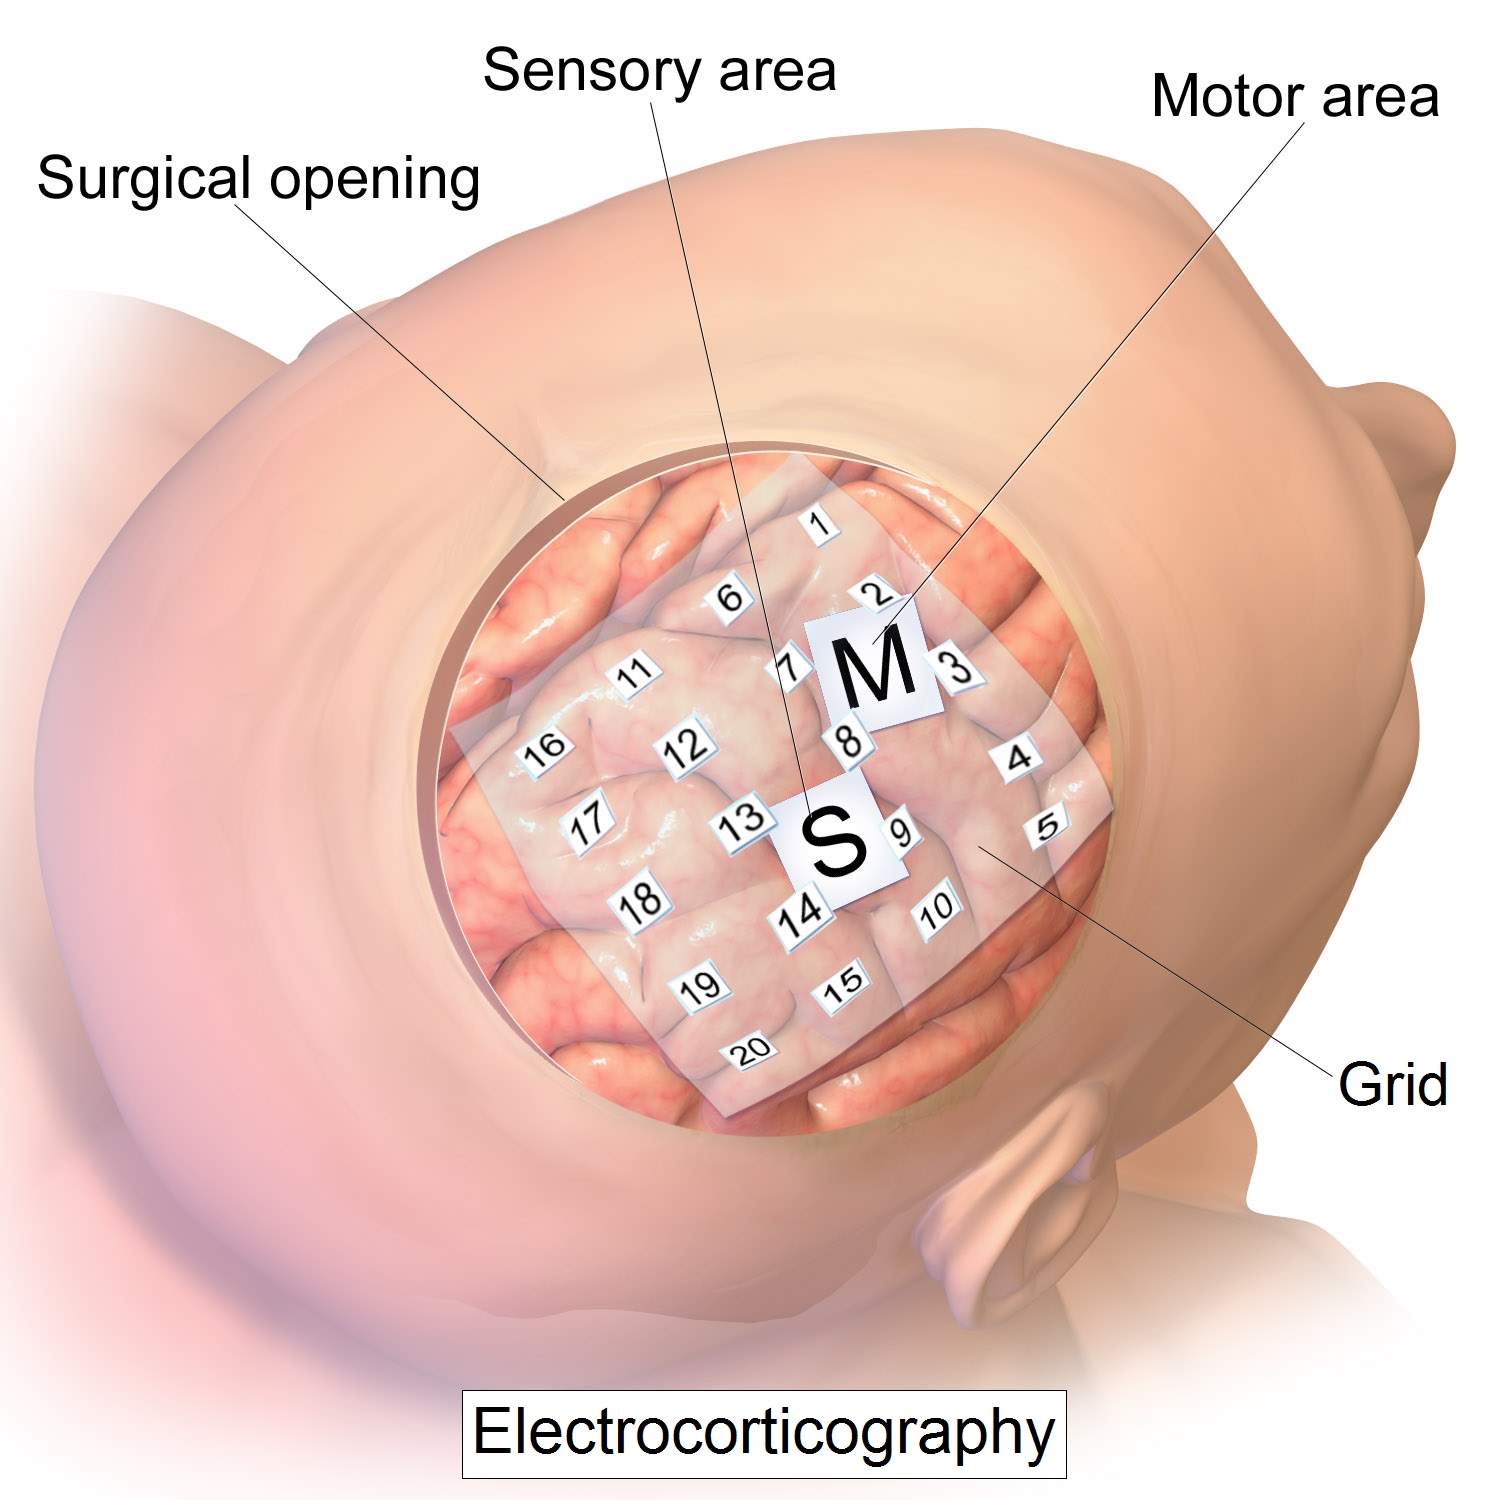
\includegraphics[width=.3\textwidth]{eocg.png}
	\end{center}
	\begin{itemize}
		\item Predict hand motion based on ECoG measurements.
		\item \textbf{Model order:} predict movement at time $t$ using brain signals at time $t,t-1, \ldots, t-q$ for varying values of $q$. 
	\end{itemize} 
\end{frame}



\begin{frame}
	\frametitle{model selection}
	The more \textbf{complex} our model class the better our loss:
	\begin{center}
		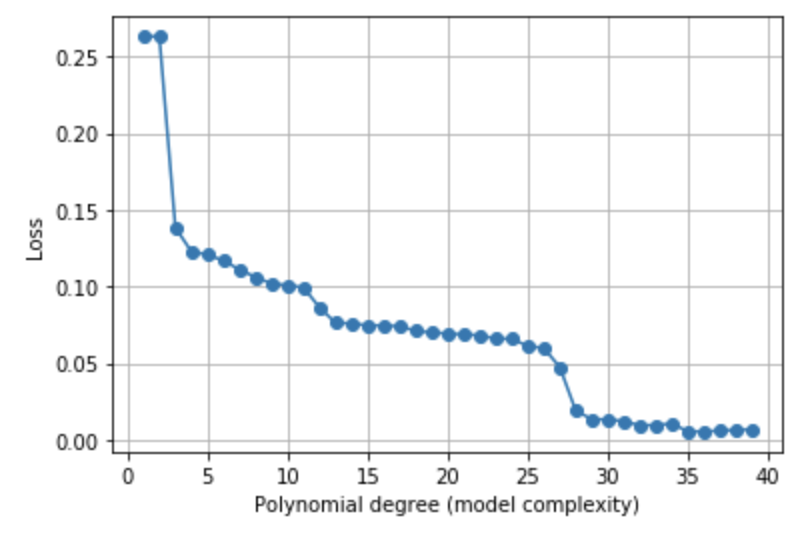
\includegraphics[width=.5\textwidth]{loss.png}
		
		\textbf{\alert{So \emph{training loss} alone is not usually a good metric for model selection.} Small loss does not imply \emph{generalization.}} 
	\end{center}
\end{frame}

\begin{frame}
	\frametitle{train-test paradigm}
	\textbf{Better approach:} Evaluate model on fresh \emph{test data} which was not used during training.
	
	\textbf{Test/train split:}
	\begin{itemize}
		\item Given data set $(\bv{X}, \bv{y})$, split into two sets $(\bv{X}_{\text{train}}, \bv{y}_{\text{train}})$ and $(\bv{X}_{\text{test}}, \bv{y}_{\text{test}})$.
		\item Train $q$ models $f^{(1)}, \ldots, f^{(q)}$ by finding parameters which minimize the loss on $(\bv{X}_{\text{train}}, \bv{y}_{\text{train}})$.
		\item Evaluate loss of each trained model on $(\bv{X}_{\text{test}}, \bv{y}_{\text{test}})$.
	\end{itemize}
\begin{center}
	\small
	Sometimes you will see the term \textbf{\alert{validation set}} instead of test set. Sometimes there will be both: use validation set for choosing the model, and test set for getting a final performance measure. 
\end{center}
\end{frame}

\begin{frame}
	\frametitle{train-test paradigm}

	\begin{center}
		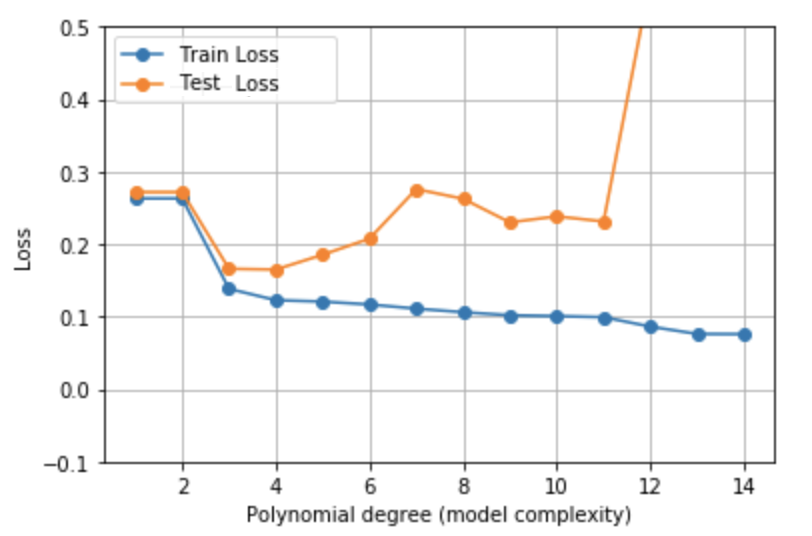
\includegraphics[width=.6\textwidth]{generalization.png}
	\end{center}
	\begin{itemize}
		\item \textbf{Train loss} continues to decrease as model complexity grows.
		\item \textbf{Test loss} ``turns around'' once our model gets too complex. Minimized around degree $3-4$.
	\end{itemize}
\end{frame}

\begin{frame}
	\frametitle{train-test paradigm}
	\textbf{Typical train-test split:} 70-90\% / 10-30\%.
	Trade-off between between optimization of model parameters and better estimate of model performance. 
	
	\textbf{Cross-validation} can offer a better trade off:
	\begin{center}
		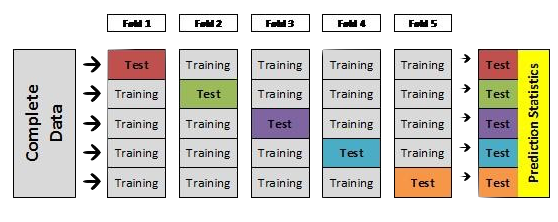
\includegraphics[width=.7\textwidth]{crossval.png}
	\end{center}
	
\end{frame}

\begin{frame}
	\frametitle{train-test intuition}
	\textbf{Intuition:} Models which perform better on the test set will \alert{\textbf{generalize}} better to future data. 
	
	\vspace{2em}
	 \textbf{Goal:} Introduce a little bit of formalism to better understand what this means. What is ``future'' data?
\end{frame}




\begin{frame}
	\frametitle{statistical learning model}
	\textbf{Statistical Learning Model:}
	\begin{itemize}
		\item Assume each data example is randomly drawn from some distribution $(\bv{x},y)\sim \mathcal{D}$.
	\end{itemize}

	\begin{center}
		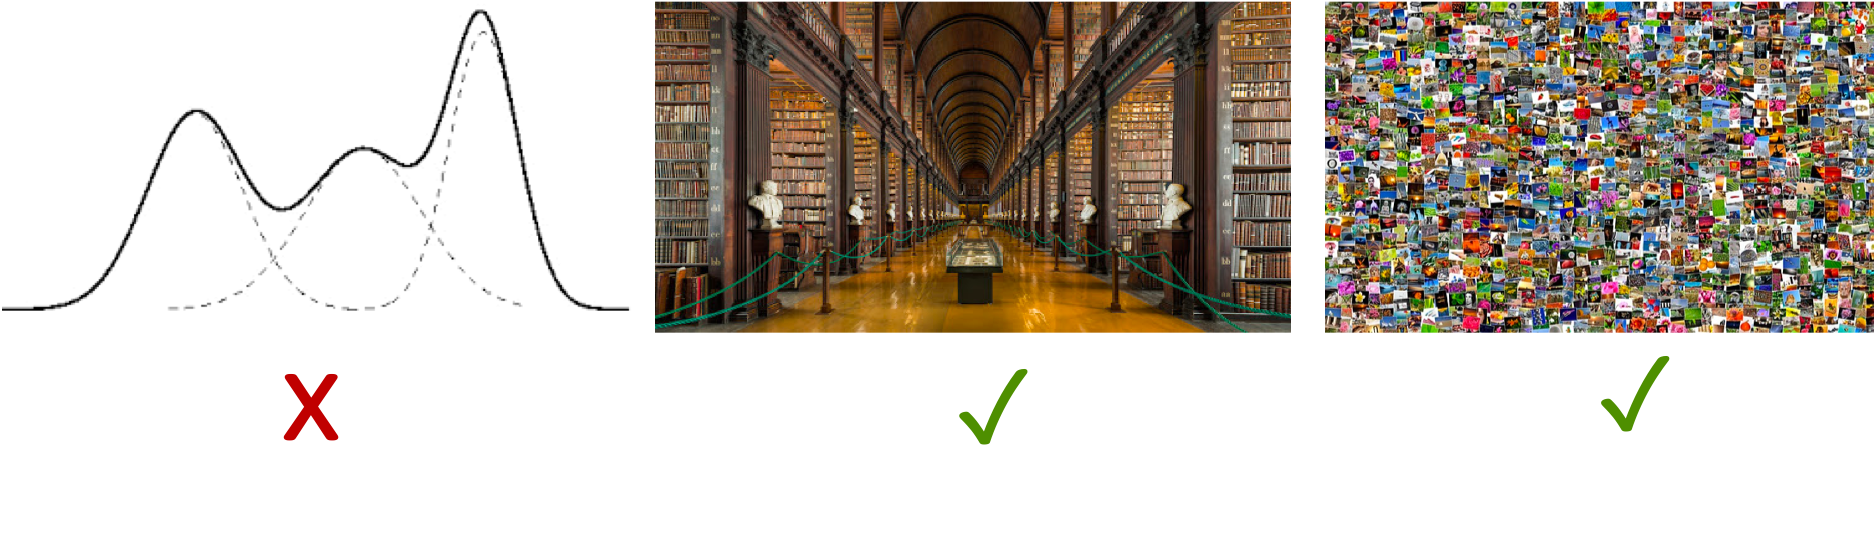
\includegraphics[width=.9\textwidth]{distributions.png}
		
		This is not a simplifying assumptions! The distribution could be arbitrarily complicated. 
	\end{center}
\end{frame}

\begin{frame}
	\frametitle{risk}
		\textbf{Statistical Learning Model:}
	\begin{itemize}
		\item Assume each data example is randomly drawn from some distribution $(\bv{x},y)\sim \mathcal{D}$.
		\item Define the \alert{\textbf{Risk}} of a model/parameters:
		\begin{align*}
		R(f,\bs{\theta}) = \E_{(\bv{x},y)\sim\mathcal{D}} \left[L\left(f(\bv{x},\bs{\theta}) - y\right) \right]
		\end{align*}
		here $L$ is some loss function (e.g. $L(z) = |z|$ or $L(z) = z^2$).
	\end{itemize}
	
	\begin{center}
		\textbf{Goal:} Find model $f \in \{f^{(1)}, \ldots, f^{(q)}\}$ and parameter vector $\bs{\theta}$ to minimize the $R(f,\bs{\theta})$.
	\end{center}
\end{frame}

\begin{frame}
	\frametitle{risk}
	\begin{itemize}
		\item \textbf{(Population) Risk}: 
		\begin{align*}
			R(f,\bs{\theta}) = \E_{(\bv{x},y)\sim\mathcal{D}} \left[L\left(f(\bv{x},\bs{\theta}) - y\right) \right]
		\end{align*}
		\item \textbf{Empirical Risk}: Draw $(\bv{x}_1,y_1), \ldots, (\bv{x}_n,y_n) \sim\mathcal{D}$
		\begin{align*}
			R_E(f,\bs{\theta}) = \frac{1}{n}\sum_{i=1}^n L\left(f(\bv{x},\bs{\theta}) - y\right)
		\end{align*}
	\end{itemize}
	Minimizing training loss is the same as minimizing the \emph{empirical risk} on the \emph{training data}. 
	
	Often called \alert{\textbf{empirical risk minimization}}.
\end{frame}


\begin{frame}
	\frametitle{empirical risk}
	For any \emph{fixed} model $f$ and parameters $\bs{\theta}$,
	\begin{align*}
		\E\left[R_E(f,\bs{\theta})\right] = R(f,\bs{\theta}).
	\end{align*}
	Only true if $f$ and $\bs{\theta}$ are chosen \textit{without looking at the data used to compute the empirical risk.}
\end{frame}

\begin{frame}
	\frametitle{model selection}
	\begin{itemize}
		\item Train $q$ models $(f^{(1)}, \bs{\theta}_1^*), \ldots, (f^{(q)}, \bs{\theta}_q^*)$.
		\item For each model, compute empirical risk $R_E(f^{(i)}, \bs{\theta}_i^*)$ using \emph{test data}. 
		\item Since we assume our original dataset was drawn independently from $\mathcal{D}$, so is the random test subset.
	\end{itemize}

\begin{center}
	No matter how our models were trained or how complex they are, $R_E(f^{(i)}, \bs{\theta}_i^*)$ is an \emph{unbiased estimate} of the true risk $R(f^{(i)}, \bs{\theta}_i^*)$ for every $i$. Can use it to distinguish between models.
\end{center}
\end{frame}

\begin{frame}
	\frametitle{adaptive data analysis}
	\begin{center}
		\textbf{Slight caveat: \alert{This is typically not how machine learning or scientific discover works in practice!}}
	\end{center}
	
	\textbf{Typical workflow:}
	\begin{itemize}
		\item Train a class of models.
		\item Test.
		\item Adjust class of models.
		\item Test. 
		\item Adjust class of models.
		\item Cont...
	\end{itemize}
	Final model implicitly depends on test set because performance on the test set guided how we changed our model. 
\end{frame}

\begin{frame}
	\frametitle{adaptive data analysis}
	\begin{center}
		\textbf{Popularity of ML benchmarks and competitions leads to adaptivity at a massive scale.}
		
		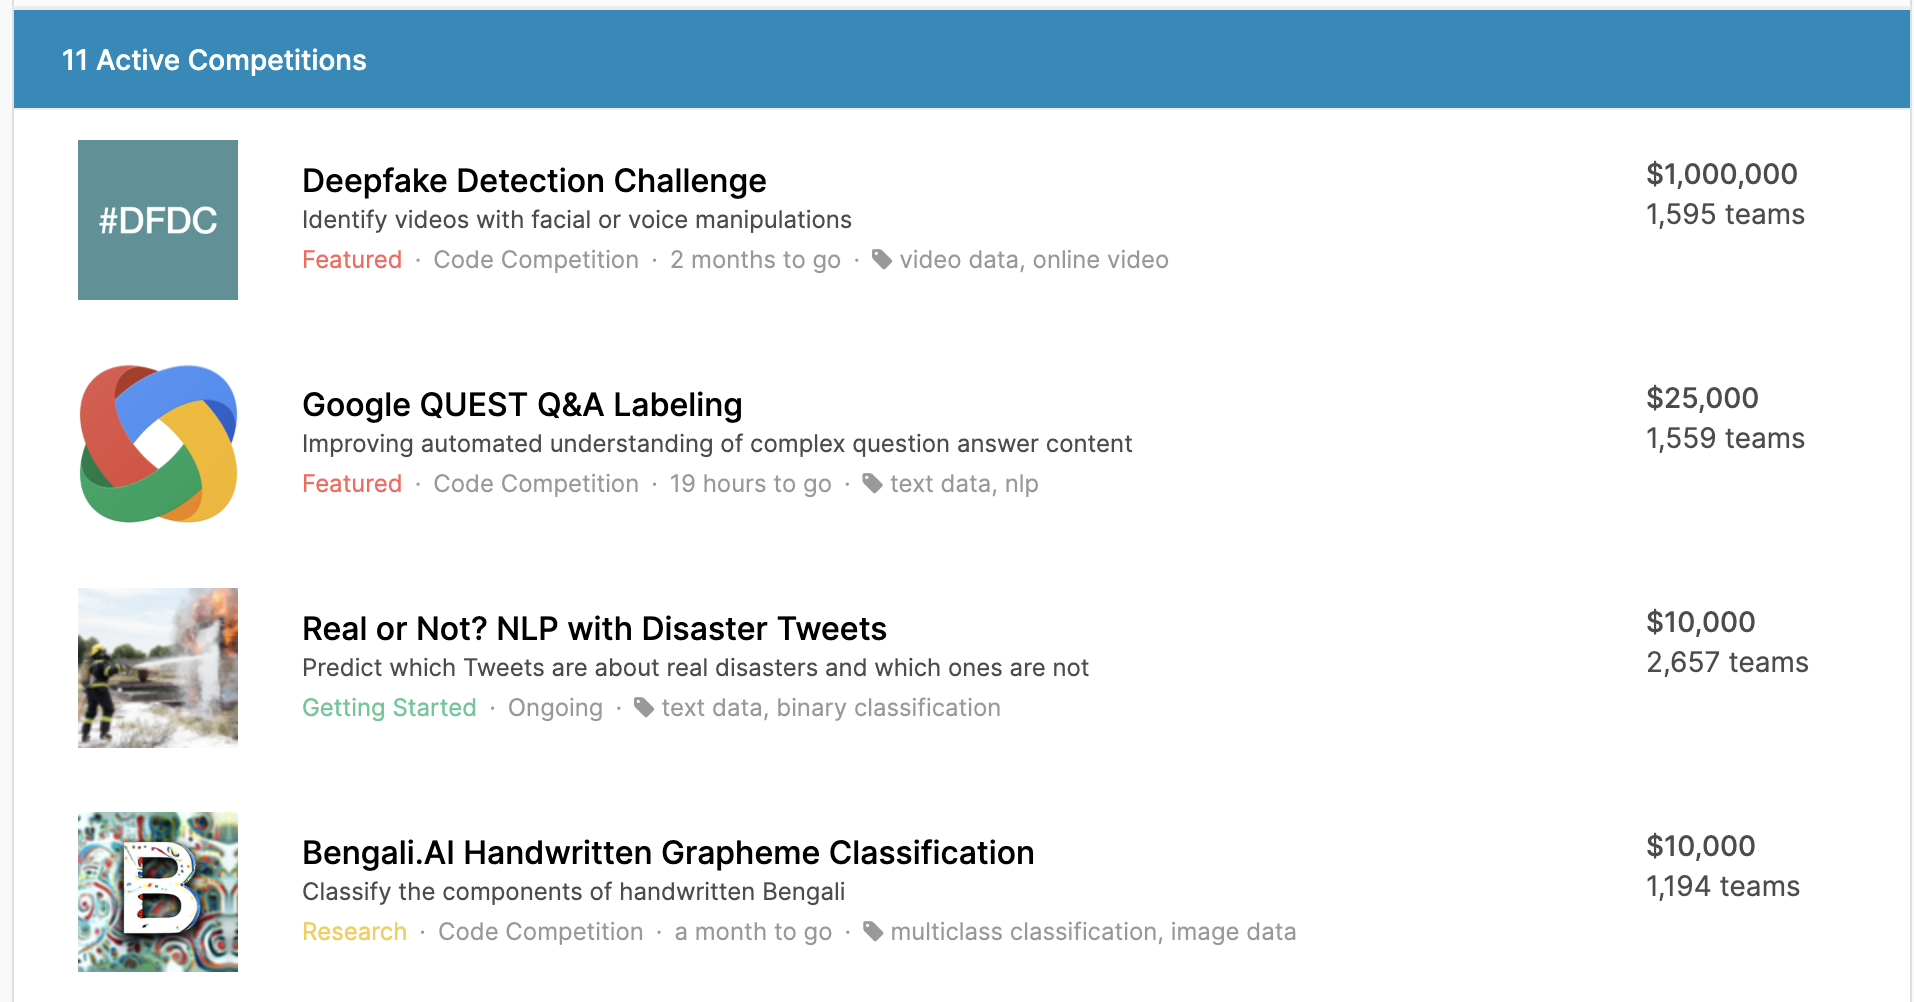
\includegraphics[width=.7\textwidth]{kaggle.png}
		
		\vspace{-1em}
		Kaggle (various competitions)
		
		\vspace{1em}
		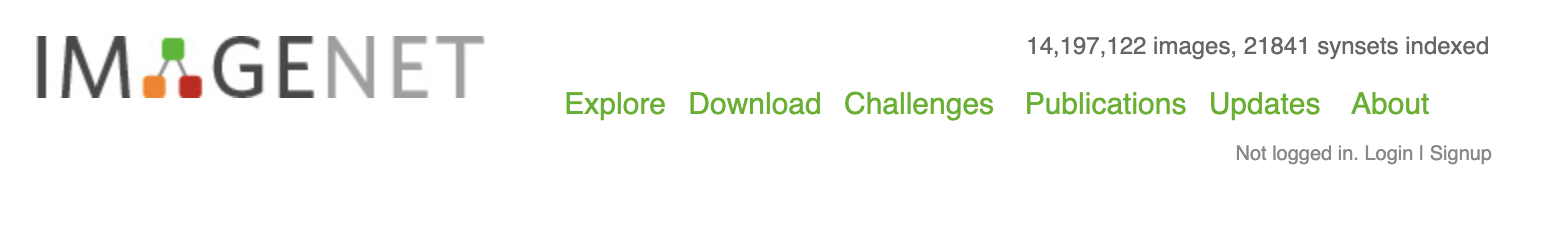
\includegraphics[width=.7\textwidth]{imagenet.png}
		
		\vspace{-1em}
		Imagenet (image classification and categorization)
	\end{center}
	
\end{frame}

\begin{frame}
	\frametitle{adaptive data analysis}
	\begin{center}
			\textbf{Is adaptivity a problem? Does it lead to over-fitting? How much? How can we prevent it?} All current research.
			
			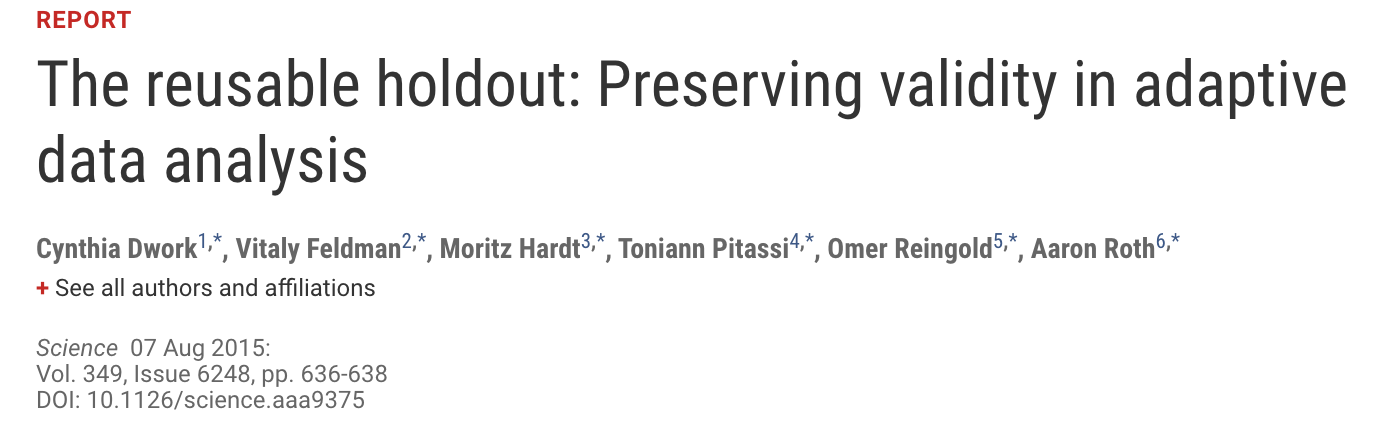
\includegraphics[width=.8\textwidth]{holdout.png}

			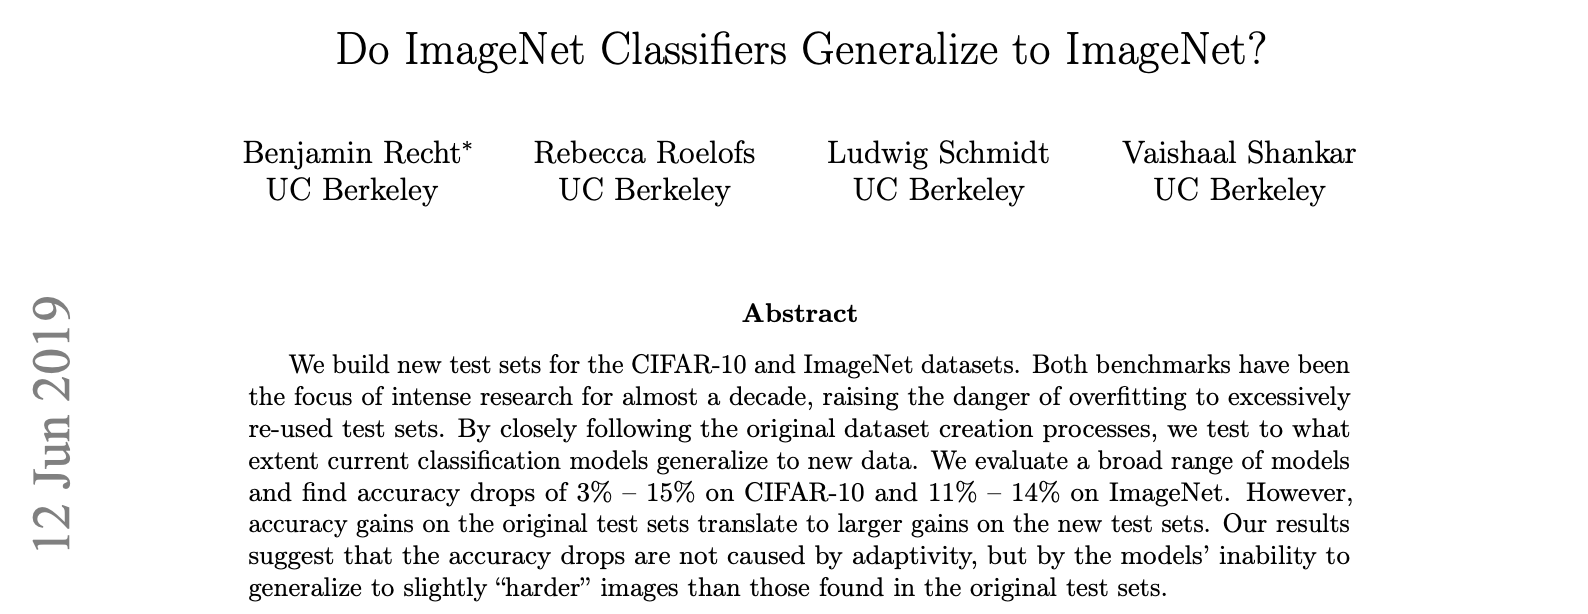
\includegraphics[width=.8\textwidth]{adaptivity.png}
	\end{center}
\end{frame}

\begin{frame}[standout]
	\begin{center}
		\large regularization
	\end{center}
\end{frame}

\begin{frame}
	\frametitle{over-parameterized models}
	In all the model selection examples we've discussed we had full control over the complexity of the model: could range from \emph{underfitting} to \emph{overfitting}. 
		
	\begin{center}
		In practice, you often don't have this freedom. Even the \emph{most basic model} will overfit. 
		
		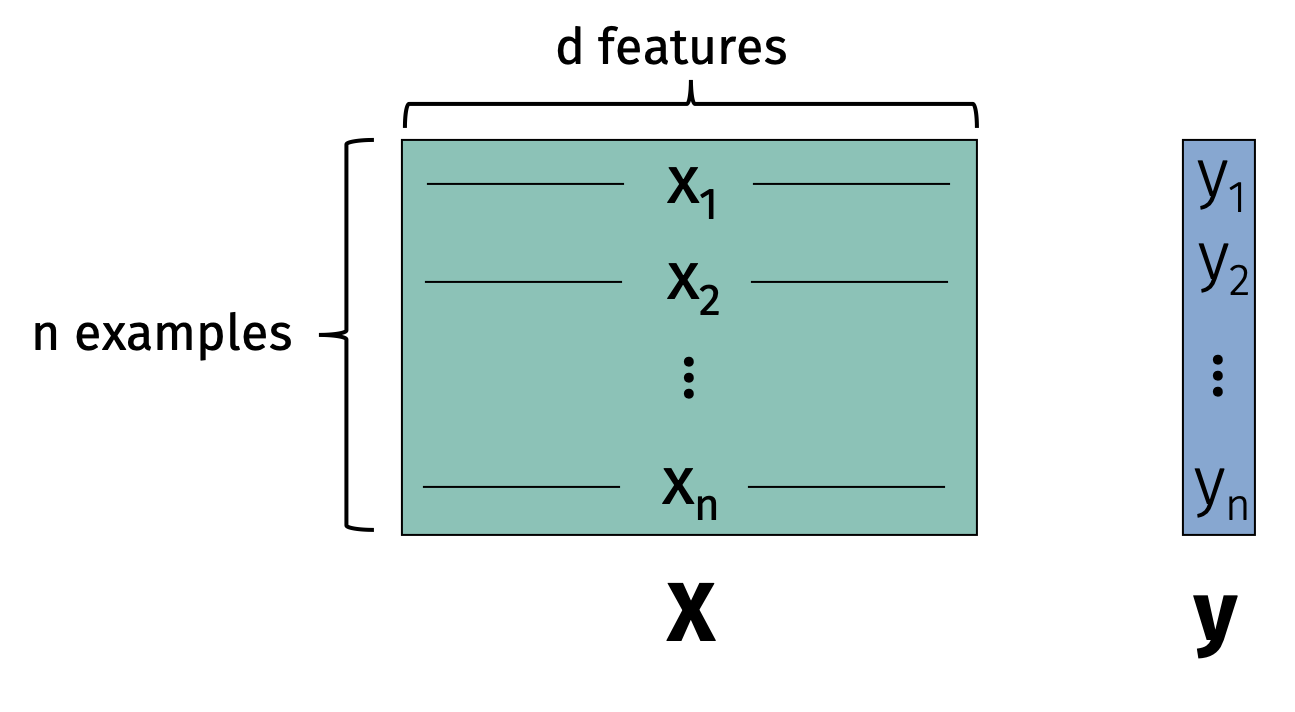
\includegraphics[width=.5\textwidth]{overparameterized.png}
		
		\textbf{Example:} Linear regression model where $d \geq n$. Can always find $\bs{\beta}$ so that $\bv{X}\bs{\beta} = \bv{y}$ exactly. 
	\end{center}
\end{frame}

\begin{frame}
	\frametitle{feature selection}
	Select some subset of features to use in model:
	\begin{center}
			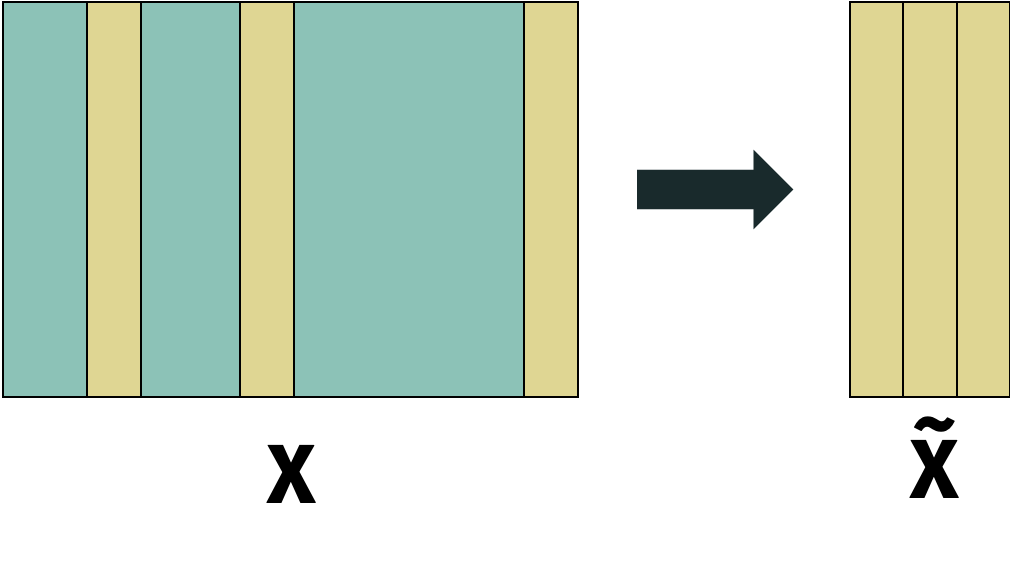
\includegraphics[width=.5\textwidth]{feature_selection.png}
	\end{center}
	\textbf{Filter method:} Compute some metric for each feature, and select features with highest score. 
	\begin{itemize}
		\item Example: compute loss/$R^2$ value when each feature in $\bv{X}$ is used in single variate regression. 
	\end{itemize} 
\begin{center}
	\alert{\textbf{Any potential limitations of this approach?}}
\end{center}
\end{frame}

\begin{frame}
	\frametitle{feature selection}
	\textbf{Exhaustive approach:} Pick best subset of $q$ features. 
	
	\textbf{Faster approach:} Greedily select $q$ features. 
	
	\textbf{Stepwise Regression:}
	\begin{itemize}
		\item \textbf{Forward:} Step 1: pick single feature that gives lowest loss. Step $k$: pick feature that when combined with previous $k-1$ chosen features gives lowest loss.
		\item \textbf{Backward:} Start with all of the features. Greedily eliminate those which have least impact on model performance.
	\end{itemize}

	Feature selection deserves more than two slides, but we won't go into too much more detail!
\end{frame}

\begin{frame}
	\frametitle{alternative approach}
	\textbf{Regularization:}
	Explicitly discourage overfitting by adding a \emph{regularization penalty} to the loss minimization problem.  
	\begin{align*}
		\min_{\bs{\theta}} \left[ L(\bs{\theta}) \alert{+ Reg(\bs{\theta})} \right].
	\end{align*}
	
	\textbf{Example:} Least squares regression. $L(\bs{\beta}) = \|\bv{X}\bs{\beta} - \bv{y}\|_2^2$.
	\begin{itemize}
		\item Ridge regression ($\ell_2$): \alert{$Reg(\bs{\beta}) = \lambda \|\bs{\beta}\|_2^2$}
		\item LASSO (least absolute shrinkage and selection operator) ($\ell_1$): \alert{$Reg(\bs{\beta}) = \lambda \|\bs{\beta}\|_1$}
		\item Elastic net: \alert{$Reg(\bs{\beta}) = \lambda_1 \|\bs{\beta}\|_1 + \lambda_2 \|\bs{\beta}\|_2^2$}
	\end{itemize}
\end{frame}

\begin{frame}
	\frametitle{ridge regularization}
	\begin{center}
		Ridge regression: $\min_{\bs{\beta}} \|\bv{X}\bs{\beta} - \bv{y}\|_2^2 + \lambda \|\bs{\beta}\|_2^2$.
	\end{center}
\begin{itemize}
	\item As $\lambda \rightarrow \infty$, we expect $\|\bs{\beta}\|_2^2 \rightarrow 0$ and $\|\bv{X}\bs{\beta} - \bv{y}\|_2^2 \rightarrow \|\bv{y}\|_2^2$.
	\item Feature selection methods attempt to set many coordinates in $\bs{\beta}$ to 0. Ridge regularizations encourages coordinates to be small. 
\end{itemize}
\vspace{-1em}
	\begin{center}
	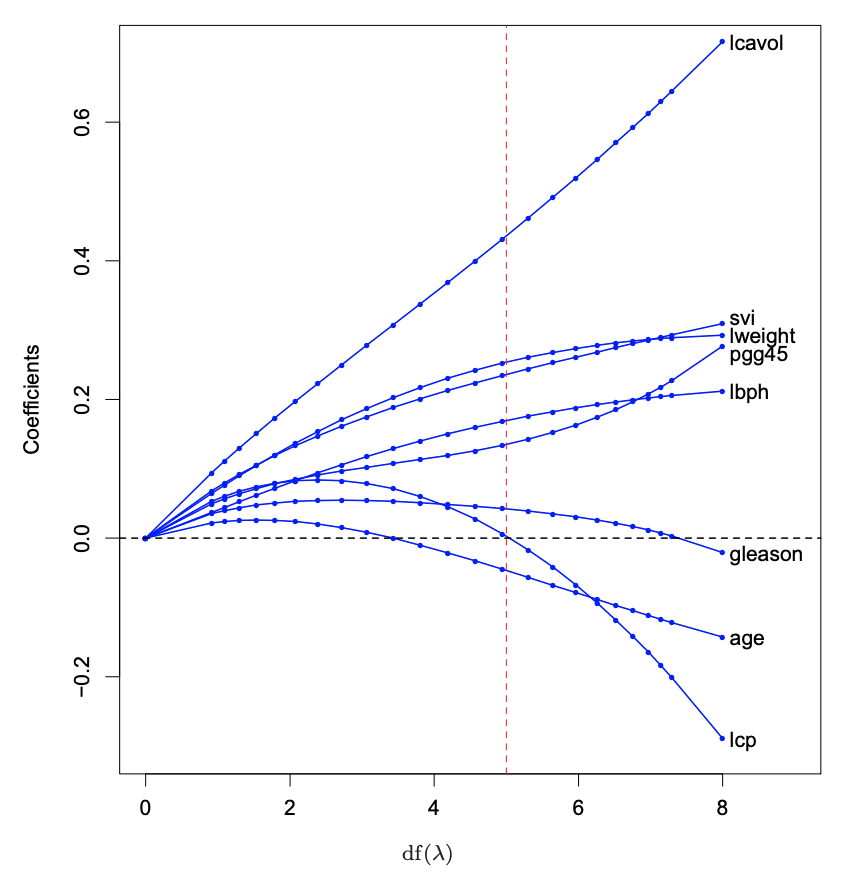
\includegraphics[width=.4\textwidth]{ridge_coeff.png}
	\end{center}
\end{frame}

\begin{frame}
	\frametitle{ridge regularization}
	\begin{center}
		Ridge regression: $\min_{\bs{\beta}} \|\bv{X}\bs{\beta} - \bv{y}\|_2^2 + \lambda \|\bs{\beta}\|_2^2$.
	\end{center}
	\begin{itemize}
		\item Can be viewed as shrinking the size of our model class. Relaxed version of $\min_{\bs{\beta}: \|\bs{\beta}\|_2^2 < c} \|\bv{X}\bs{\beta} - \bv{y}\|_2^2$. Which won't have a solution at zero for all $\bv{y}$, even when over-parameterized.
		
		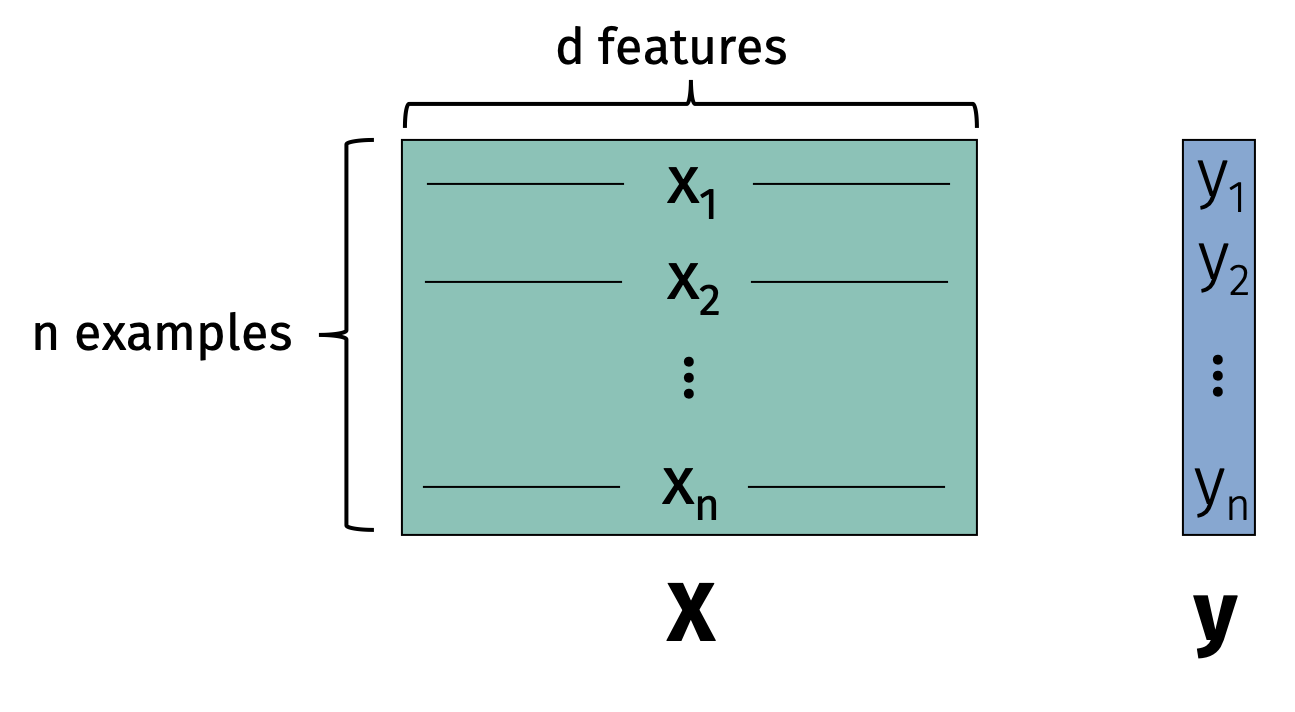
\includegraphics[width=.5\textwidth]{overparameterized.png}
		
		\item Method is \emph{not invariant} to data scaling. Typically when using regularization we mean center and scale columns to have unit variance.
	\end{itemize}
\end{frame}

\begin{frame}
	\frametitle{lasso regularization}
		\begin{center}
		Lasso regularization: $\min_{\bs{\beta}} \|\bv{X}\bs{\beta} - \bv{y}\|_2^2 + \lambda \|\bs{\beta}\|_1$.
	\end{center}
	\begin{itemize}
		\item As $\lambda \rightarrow \infty$, we expect $\|\bs{\beta}\|_1 \rightarrow 0$ and $\|\bv{X}\bs{\beta} - \bv{y}\|_2^2 \rightarrow \|\bv{y}\|_2^2$.
		\item Typically encourages subset of $\bs{\beta}_i$'s to go to zero, in contrast to ridge regularization.
	\end{itemize}
	\vspace{-1em}
	\begin{center}
		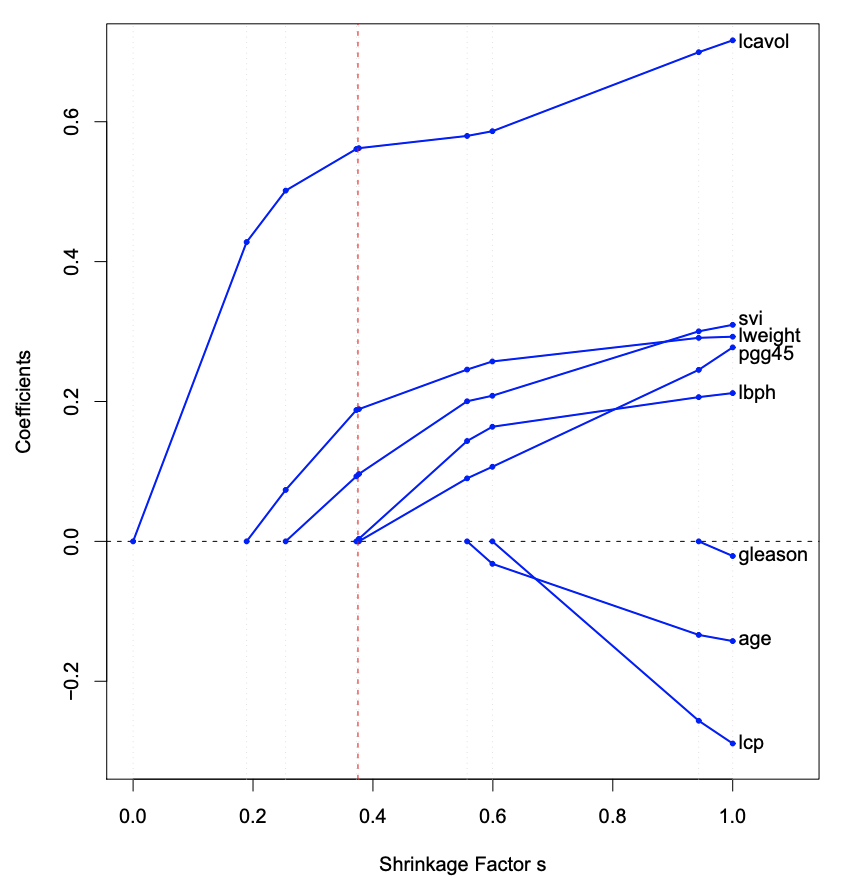
\includegraphics[width=.4\textwidth]{lasso_coeffs.png}
	\end{center}
\end{frame}

\begin{frame}
	\frametitle{lasso regularization}
	\textbf{Pros:}
	\begin{itemize}
		\item Simpler, more interpretable model.
		\item More intuitive reduction in model order.
	\end{itemize}

	\textbf{Cons:}
\begin{itemize}
	\item No closed form solution because $\|\bs{\beta}\|_1$ is not differentiable. 
	\item Can be solved with iterative methods, but generally not as quickly as ridge regression.
\end{itemize}
	
\end{frame}

\begin{frame}
	\frametitle{regularization}
	\textbf{Notes:}
	\begin{itemize}
		\item Model selection/cross validation used to choose optimal scaling $\lambda$ on $\lambda \|\bs{\beta}\|_2^2$ or $\lambda \|\bs{\beta}\|_1$. 
		\item Often grid search for best parameters is performed in ``log space''. E.g. consider $[\lambda_1, \ldots,\lambda_q] = 1.5^{[-4,-3,-2,-1,-0,1,2,3,4]}$. 
	\end{itemize}
	
\end{frame}

\end{document} 








